\chapter{Visualização e representação de dados espaciais}

\pagestyle{fancy}

Visualizar a informação geográfica é parte fundamental do trabalho com SIG. Embora alguns dados já incluam sua forma própria de representação — como imagens de satélite, ortofotos ou serviços de mapas —, no SIG geralmente é o usuário quem define como o dado será representado. Ou seja, o usuário de SIG \textbf{assume o papel de cartógrafo}, devendo, portanto, conhecer os fundamentos utilizados na criação de mapas.

Além das ferramentas e conceitos clássicos da cartografia, os SIG incorporam elementos da chamada \textbf{visualização científica}, como a \textbf{interatividade} e a \textbf{representação de dados multidimensionais}. Esse novo enfoque, mais rico que o da cartografia tradicional, é conhecido como \textbf{geovisualização}.

Neste capítulo, veremos as ideias fundamentais da visualização de dados, abordando tanto sua aplicação na cartografia tradicional quanto em SIGs e geovisualização.

\section{Conceitos básicos de visualização}

Sempre que visualizamos informação geográfica — em um mapa impresso ou em uma tela de computador — utilizamos uma forma de \textbf{linguagem visual}.

O estudo dos signos de uma linguagem é chamado de \textbf{semiologia}. Quando aplicada à linguagem visual, temos a \textbf{semiologia gráfica}, que define uma gramática visual para compreender como os elementos gráficos transmitem a informação desejada.

\subsection{As variáveis visuais}

Existem diferentes propriedades dos elementos visuais que podemos usar para comunicar informação. Cada uma é mais ou menos adequada dependendo do tipo de dado representado.

\begin{figure}[!hbt]
\centering
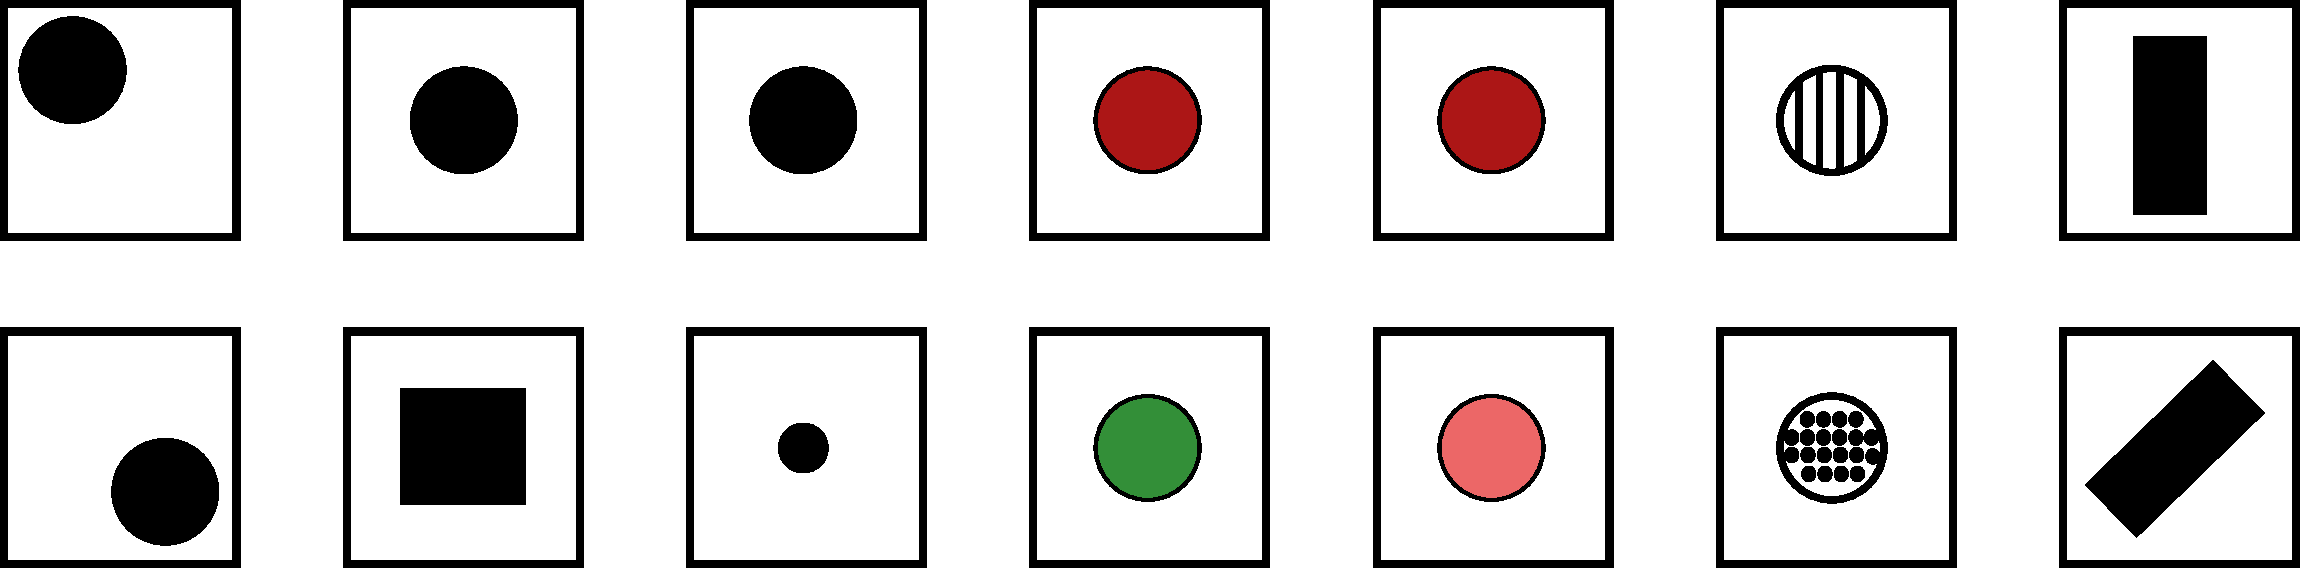
\includegraphics[width=\columnwidth]{Visualizacao/VariablesVisuales.pdf}
\caption{\small Exemplos de uso das variáveis visuais: posição, forma, tamanho, tom, valor, textura e orientação.}
\label{Fig:VariablesVisuales} 
\end{figure}

Essas propriedades são chamadas de \textbf{variáveis visuais}. Elas se aplicam aos elementos geométricos básicos da representação. São: posição, forma, tamanho, textura, cor e orientação (Figura~\ref{Fig:VariablesVisuales}).

- A \textbf{posição} não é livre em mapas, pois deve respeitar a localização geográfica real.
- A \textbf{forma} refere-se ao contorno dos símbolos, especialmente em pontos. Seu uso em linhas e polígonos é limitado.
- O \textbf{tamanho} aplica-se diretamente em pontos (maior símbolo = maior valor) e linhas (espessura). Para polígonos, aplica-se mais à textura.
- A \textbf{textura} envolve padrões internos nos símbolos, como hachuras.
- A \textbf{cor} é a variável visual mais poderosa. Divide-se em:
  - \textbf{Tom}: nome da cor (ex: vermelho, azul)
  - \textbf{Valor}: claridade ou escuridão da cor
- A \textbf{orientação} altera o ângulo de símbolos ou padrões.

\subsection{Propriedades das variáveis visuais}

Cada variável visual pode ter uma ou mais destas 4 propriedades:

\begin{itemize}
	\item \textbf{Associativa}: não altera o destaque de um símbolo
	\item \textbf{Seletiva}: permite categorizar os símbolos
	\item \textbf{Ordenada}: transmite uma ordem ou sequência
	\item \textbf{Quantitativa}: expressa proporções ou quantidades
\end{itemize}

Essas propriedades estão organizadas em \emph{níveis de organização}. A Tabela~\ref{Tabla:PropiedadesVariablesVisuales} resume como cada variável se comporta:

\begin{table}[!hbt]
\small
\centering  \label{Tabla:PropiedadesVariablesVisuales}
\begin{tabular}{p{3.6cm}ccccccc}  
 & \rotatebox{90}{\textbf{Posição}} & \rotatebox{90}{\textbf{Tamanho}} & \rotatebox{90}{\textbf{Forma}} & \rotatebox{90}{\textbf{Valor}} & \rotatebox{90}{\textbf{Tom}} & \rotatebox{90}{\textbf{Textura}} & \rotatebox{90}{\textbf{Orientação}} \\ \midrule   
\textbf{Associativa} & $\diamondsuit$ & - & $\diamondsuit$ & - & $\diamondsuit$ & $\diamondsuit$ & $\diamondsuit$ \\
\textbf{Seletiva}   & $\diamondsuit$ & $\diamondsuit$ & - & $\diamondsuit$ & $\diamondsuit$ & $\diamondsuit$ & $\diamondsuit$ \\
\textbf{Ordenada}   & $\diamondsuit$ & $\diamondsuit$ & - & $\diamondsuit$ & - & - & - \\
\textbf{Quantitativa} & $\diamondsuit$ & $\diamondsuit$ & - & - & - & - & -  \\
\bottomrule \end{tabular}
\caption{\small Resumo das propriedades das variáveis visuais.}
\end{table}

\subsection{Percepção das variáveis visuais}

A percepção de uma variável visual pode ser afetada pelo \textbf{contexto visual} — como cor de fundo, contraste com vizinhos, entre outros.

Conceitos importantes:

- \textbf{Constância perceptiva}: percebemos um objeto como o mesmo, mesmo sob mudanças (ex: forma circular vista em perspectiva).
- \textbf{Contraste perceptivo}: a percepção muda mesmo que o objeto não tenha mudado.

Recomendações para minimizar erros de percepção:

- Evitar sobreposição de tamanhos diferentes
- Cuidar do contraste de valor e tom
- Usar cores com cuidado para evitar ilusões visuais (ex: vibração entre complementares)
- Estabelecer uma \textbf{hierarquia visual} clara entre elementos (Figura~\ref{Fig:JerarquiaMapa})

\begin{figure}[!hbt]
\centering
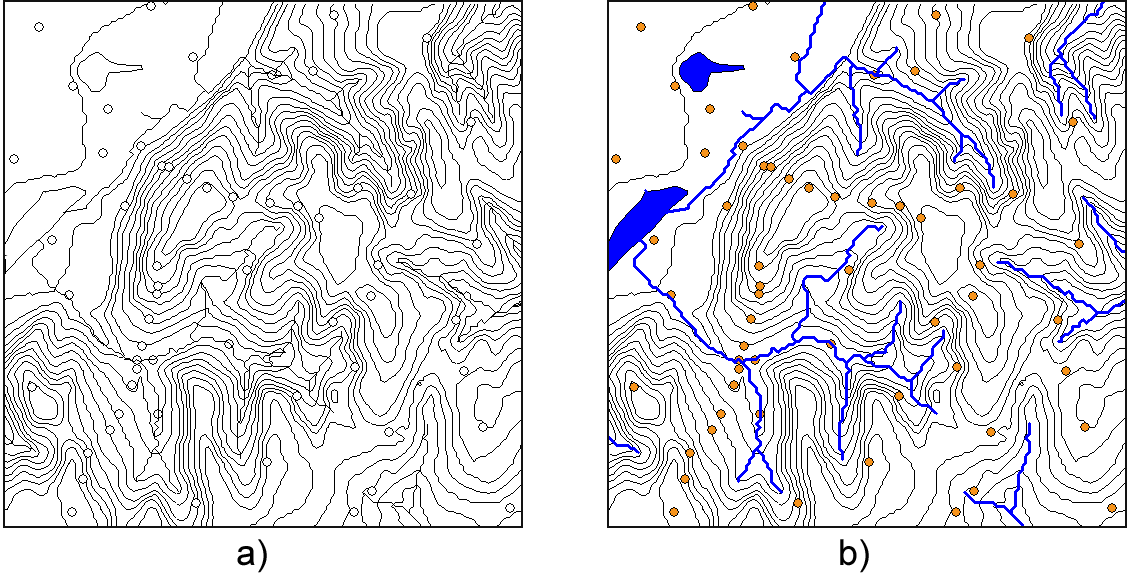
\includegraphics[width=\columnwidth]{Visualizacao/JerarquiaMapa.png}
\caption{\small Mapa com hierarquia incorreta (a) e correta (b).}
\label{Fig:JerarquiaMapa} 
\end{figure}

\section{Mapas e comunicação cartográfica}

Mapas são formas visuais de comunicar relações espaciais. São abstrações simbólicas e generalizadas da realidade.

Dois tipos principais:

\begin{itemize}
 \item \textbf{Cartografia base (topográfica)}: descreve o terreno físico
 \item \textbf{Cartografia temática}: representa uma variável específica (social, política, ambiental etc.)
\end{itemize}

Cartografia temática costuma se apoiar na cartografia base.

\subsection{Tipos de informação e representação}

Escolher a variável visual correta depende do tipo de dado:

\begin{itemize}
 \item \textbf{Nominal}: usar forma, tom ou textura
 \item \textbf{Ordinal}: requer variável com propriedade \emph{ordenada}
 \item \textbf{Intervalar e razão}: preferir \emph{tamanho}, que tem a propriedade \emph{quantitativa}
\end{itemize}

É comum agrupar valores contínuos em classes: intervalos iguais, percentis, intervalos naturais, etc. (ver Figura~\ref{Fig:TiposIntervalosClases})

\begin{figure}[!hbt]
\centering
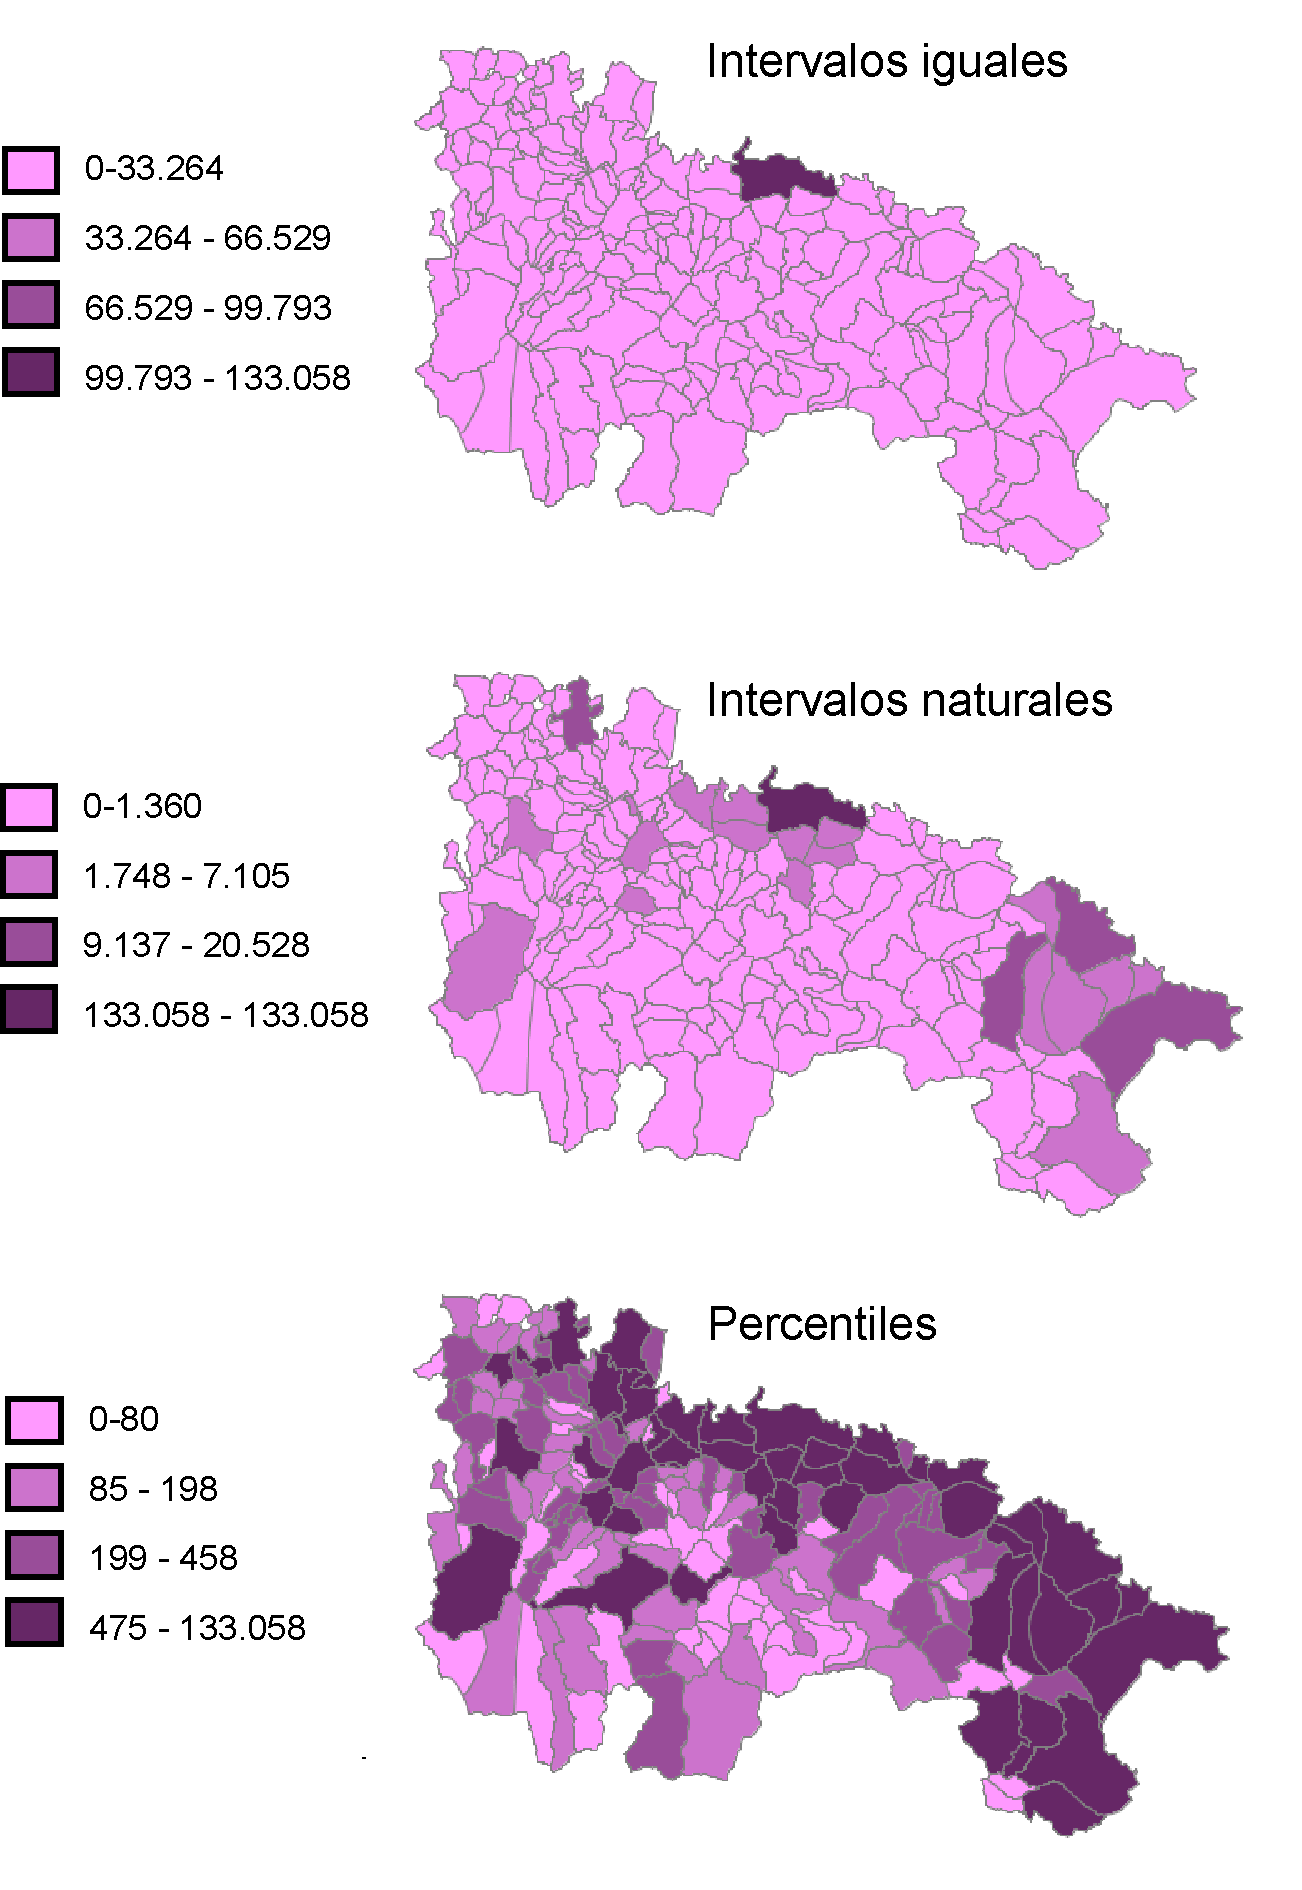
\includegraphics[width=.7\columnwidth]{Visualizacao/TiposIntervalosClases.pdf}
\caption{\small Diferenças entre métodos de classificação em mapas.}
\label{Fig:TiposIntervalosClases} 
\end{figure}

\subsection{Elementos do mapa}

Elementos comuns em mapas (Figura~\ref{Fig:ElementosMapa}):

\begin{figure}[!hbt]
\centering
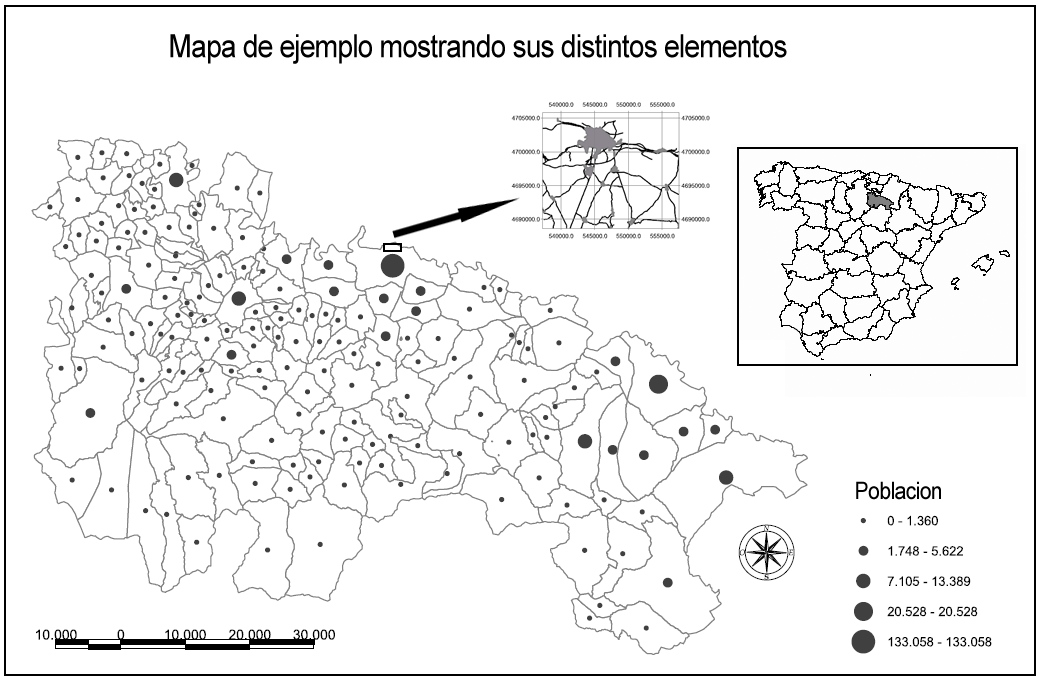
\includegraphics[width=\columnwidth]{Visualizacao/ElementosMapa.png}
\caption{\small Elementos principais de um mapa.}
\label{Fig:ElementosMapa} 
\end{figure}

\begin{itemize}
 \item Título
 \item Autor
 \item Informações complementares (ex: sistema de referência)
 \item Canevás (grade)
 \item Legenda
 \item Norte
 \item Escala (gráfica e numérica)
 \item Mapa de localização (contexto geográfico)
 \item Mapa de detalhe (zoom em áreas específicas)
\end{itemize}

\section{Tipos de mapas temáticos}

Apresentamos aqui os quatro principais tipos para variáveis quantitativas:

\subsection{Símbolos proporcionais}

Tamanho do símbolo proporcional ao valor representado.

Importante:

- Usar escalonamento discreto (classes)
- Incluir legenda clara (Figura~\ref{Fig:EjemplosLeyendaSimbolosProporcionales})

\begin{figure}[!hbt]
\centering
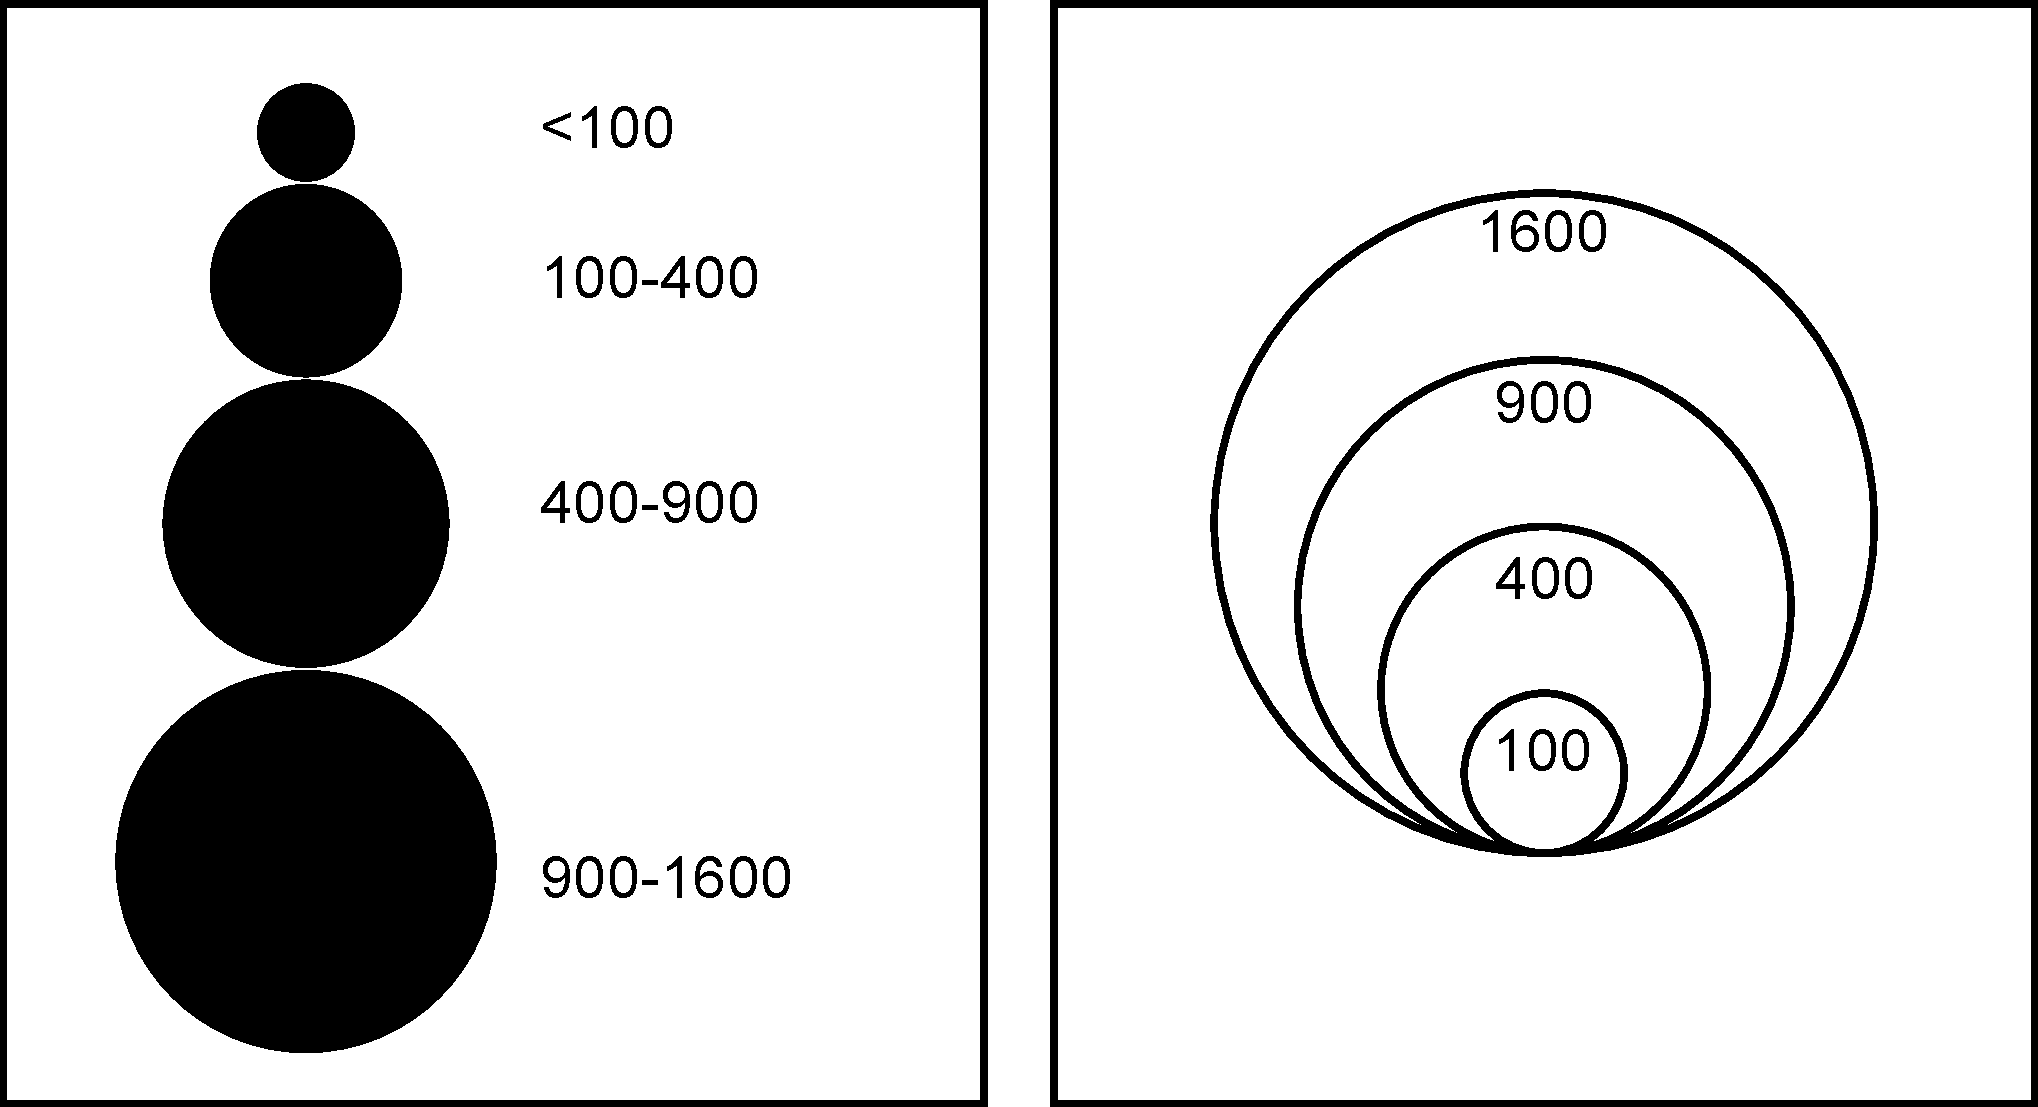
\includegraphics[width=.65\columnwidth]{Visualizacao/EjemplosLeyendaSimbolosProporcionales.pdf}
\caption{\small Exemplos de legendas para símbolos proporcionais.}
\label{Fig:EjemplosLeyendaSimbolosProporcionales} 
\end{figure}

\subsection{Mapas de pontos}

Usados para variáveis como população ou produção agrícola.

Aspectos importantes:

- Valor unitário por ponto
- Tamanho visível e adequado
- Posição coerente com distribuição esperada (Figura~\ref{Fig:MapaPontos})

\begin{figure}[!hbt]
\centering
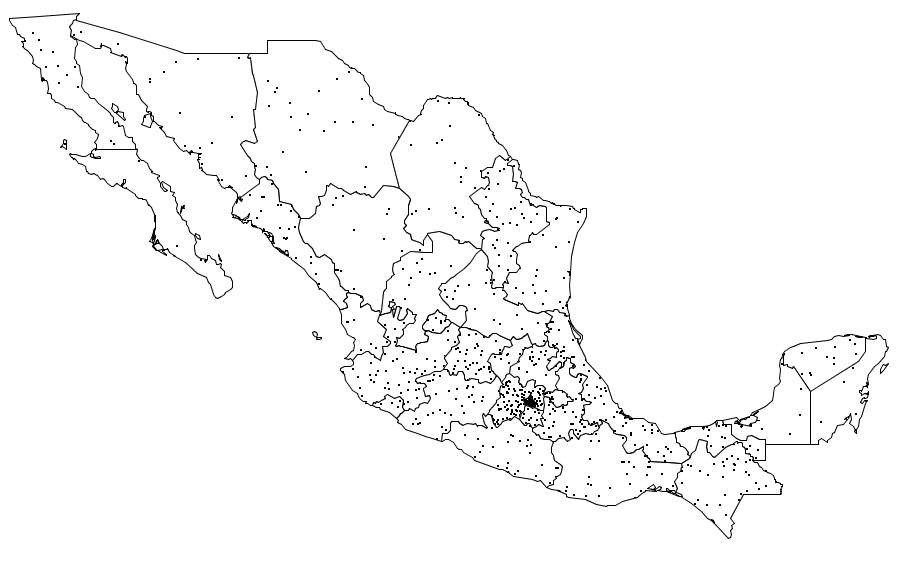
\includegraphics[width=.8\columnwidth]{Visualizacao/MapaPuntos.png}
\caption{\small Exemplo de mapa de pontos.}
\label{Fig:MapaPontos} 
\end{figure}

\subsection{Mapas de isolinhas}

Representam variáveis contínuas, como altitude ou temperatura.

- Linhas conectam pontos de mesmo valor
- \emph{Equidistância} define o espaçamento entre linhas
- Variável visual usada: espessura (para linhas principais)
- Pode-se usar coloração entre as linhas: \emph{isocoropletas} (Figura~\ref{Fig:Isolineas})

\begin{figure}[!hbt]
\centering
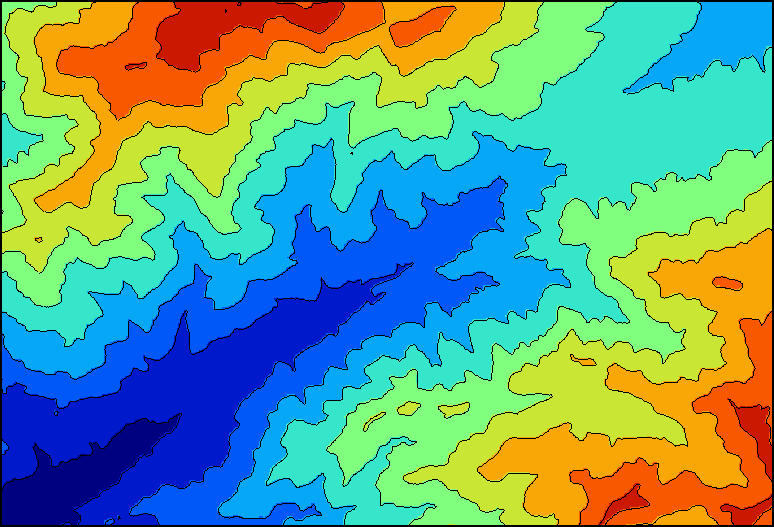
\includegraphics[width=.8\columnwidth]{Visualizacao/Isolineas.png}
\caption{\small Mapa com isolinhas e preenchimento por classes.}
\label{Fig:Isolineas} 
\end{figure}

\subsection{Mapas de coropléticas}

Usados para dados agregados por áreas.

- Representam o valor da variável por meio da cor
- Devem normalizar por área (ex: densidade populacional)
- Podem induzir interpretação errada: mudança brusca nos limites; homogeneidade interna

\section{Visualização em SIG}

Dois aspectos fundamentais:

\begin{itemize}
 \item \textbf{Composição de múltiplas camadas}
 \item \textbf{Particularidades da tela e da interatividade}
\end{itemize}

\subsection{Composição de camadas}

Importante para enriquecer a interpretação.

Boas práticas:

- Definir a \textbf{ordem de desenho}: ráster abaixo de vetores; polígonos abaixo de linhas e pontos
- Usar \textbf{transparência} quando necessário (Figura~\ref{Fig:CombinacionCapas})

\begin{figure}[!hbt]
\centering
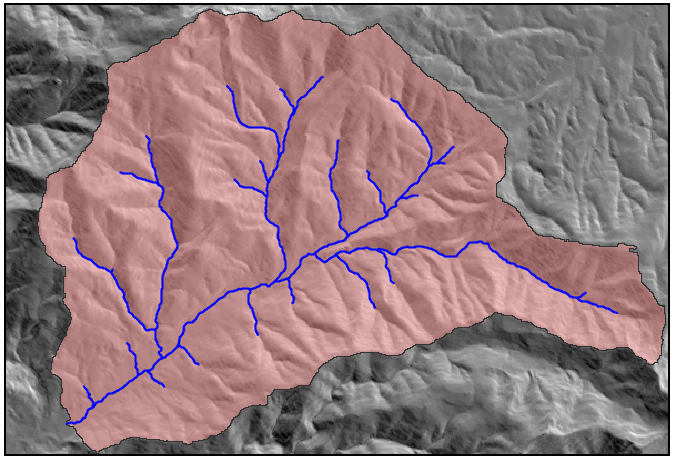
\includegraphics[width=.7\columnwidth]{Visualizacao/CombinacionCapas.png}
\caption{\small Uso de transparência para visualizar camadas sobrepostas.}
\label{Fig:CombinacionCapas} 
\end{figure}

\subsection{Particularidades da tela}

Duas limitações:

\begin{itemize}
 \item \textbf{Baixa resolução}: evitar fontes com ornamentos ou linhas muito finas
 \item \textbf{Interatividade}: o usuário pode mudar a escala (zoom)
\end{itemize}

Problemas comuns:

- Símbolos ficam ilegíveis em escalas pequenas ou exagerados em escalas grandes (Figura~\ref{Fig:ProblemasRepresentacionSimbolos})

\begin{figure}[!hbt]
\centering
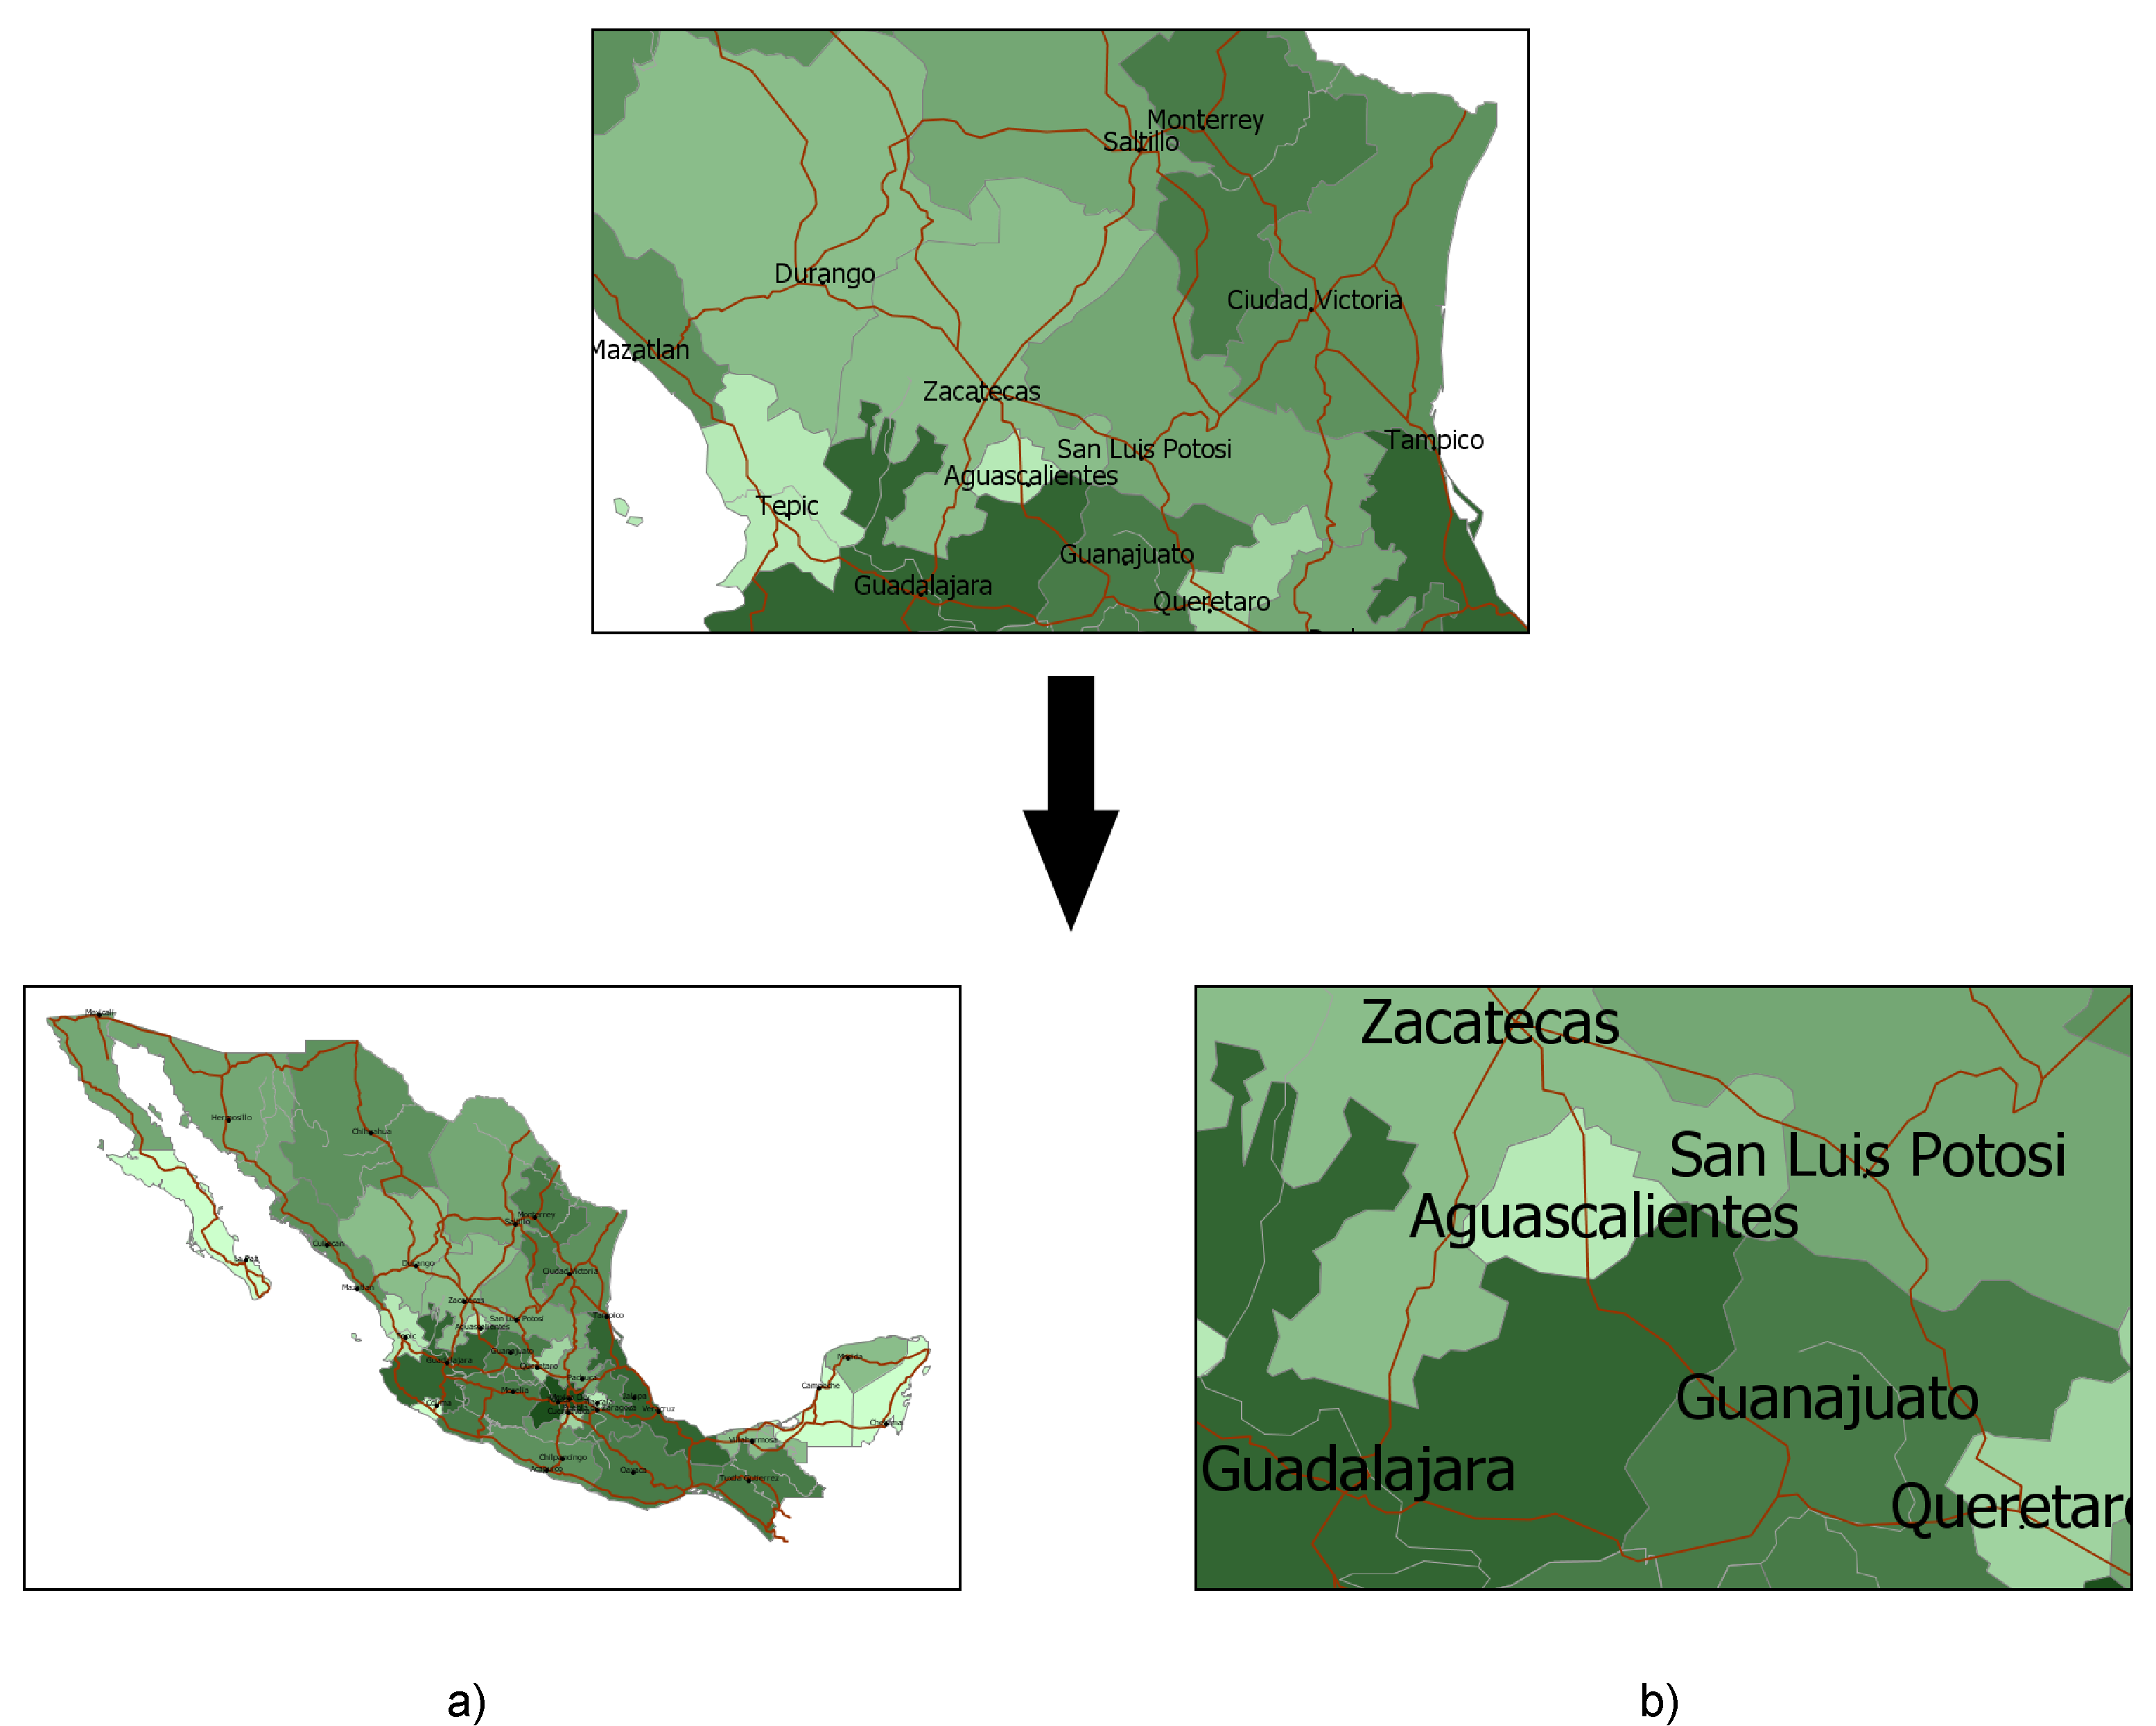
\includegraphics[width=\columnwidth]{Visualizacao/ProblemasRepresentacionSimbolos.pdf}
\caption{\small Problemas com tamanho de símbolos ao mudar a escala.}
\label{Fig:ProblemasRepresentacionSimbolos} 
\end{figure}

- Representações saturadas (Figura~\ref{Fig:RepresentacionSaturada})

\begin{figure}[!hbt]
\centering
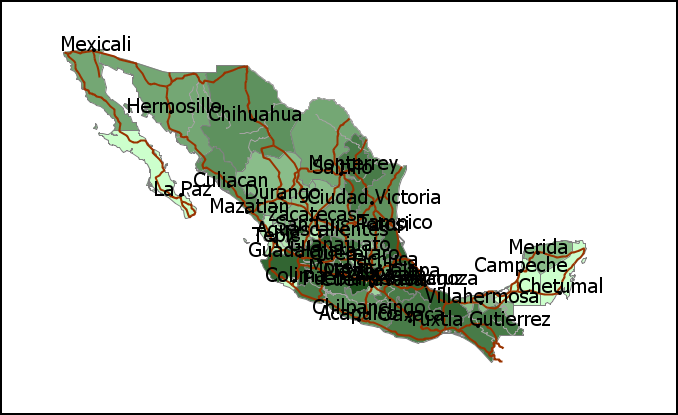
\includegraphics[width=.9\columnwidth]{Visualizacao/RepresentacionSaturada.png}
\caption{\small Representação saturada com muitos elementos.}
\label{Fig:RepresentacionSaturada} 
\end{figure}

Recomendações:

- Usar \textbf{tamanho fixo em pixels} com cautela
- Adotar abordagem \textbf{multi–escala} com diferentes camadas por escala

\pagestyle{empty}
